\section{设计概述}\label{sec:overview}

\subsection{威胁模型和信任假设}\label{subsec:threat-model}

在微服务安全计算场景中,可能的攻击方式和应对手段包括:

\begin{itemize}
    \item \textbf{系统特权态攻击}:攻击者可以通过劫持OS或者Hypervisor,通过系统的特权态获取系统中的所有信息。对此可以使用TEE进行保护,TEE的防御模型可以轻松抵御这种威胁~\cite{costan2016intel}。
    \item \textbf{网络攻击}:包括中间人攻击(MITM)和重放攻击(Replay Attack)等。这种攻击方式可以通过网络安全协议(例如TLS~\cite{8446})等方式来防御。
    \item \textbf{漏洞利用}:主要是使用系统编程语言可能带来的缓冲区溢出漏洞进行攻击。对此可以通过使用Rust语言~\cite{rust-lang}提供静态安全检查来防止。
    \item \textbf{物理攻击}:如侧信道攻击通过监测目标设备的非正常数据流或物理性能(如功耗、热量等)来获取设备中存储的敏感信息的攻击方式,这种攻击方式TEE本身无法防御,但是已有一些研究可以降低遭到攻击的可能~\cite{oleksenko2018varys}。其他物理攻击包括电磁攻击通过高能电磁波或者电磁干扰对计算机或通信设备进行攻击、拒绝服务攻击通过破坏电源等方式让服务器宕机等,这些攻击TEE也无法防御,但是这些不会造成数据泄露,应该由云服务提供商进行物理防御。
\end{itemize}

本次设计的目的是防御系统特权态攻击、网络攻击和漏洞攻击等,但是不考虑极端情况下的物理攻击。为了达到这一目的,本次设计具有以下信任假设:

\begin{itemize}
    \item \textbf{硬件可信}:硬件是可信的,即硬件不会对软件进行攻击,也不会泄露软件中的信息,硬件制造商不会在硬件中预置后门,系统不会遭到硬件攻击。
    \item \textbf{SGX可信}:SGX提供的所有机制都是可信的,包括SGX的内存加密、飞地的创建、飞地的隔离、SGX远程验证协议等。
    \item \textbf{平台可信}:项目平台本身的实现是可信的,包括微服务的运行时、通信协议的实现是正确无误的,且没有恶意代码。
    \item \textbf{Rust工具链可信}:Rust工具链是可信的,即Rust工具链在构建过程中不会对程序进行恶意修改。
    \item \textbf{开发者基本可信}:开发者不是恶意的,不会在代码中预置后门,且不会使用不安全的编程语言;但开发者的代码可能存在bug。
    \item \textbf{PaaS系统不可信}:PaaS上的Hypervisor和OS是不可信的,可能存在恶意、被劫持或系统漏洞。
    \item \textbf{网络不可信}:网络通信是不可信的,可能存在中间人攻击、重放攻击等。
          % \item \textbf{数据存储不可信}:存储到外存的数据是不可信的,可能存在数据泄露。对此其实已有一些解决方案,如对数据进行加密~\cite{}等,但是这些方案与本次研究正交,暂不考虑。
\end{itemize}

\subsection{设计总览}

基于威胁模型和信任假设,同时尽可能减小TCB并降低通信延迟,我们针对微服务安全计算场景设计了模块化的运行时、安全高效的通信协议以及微服务示例程序,共同构成了一个基于可信执行环境的安全高效的微服务计算平台。

\begin{figure}[!ht]
    \centering
    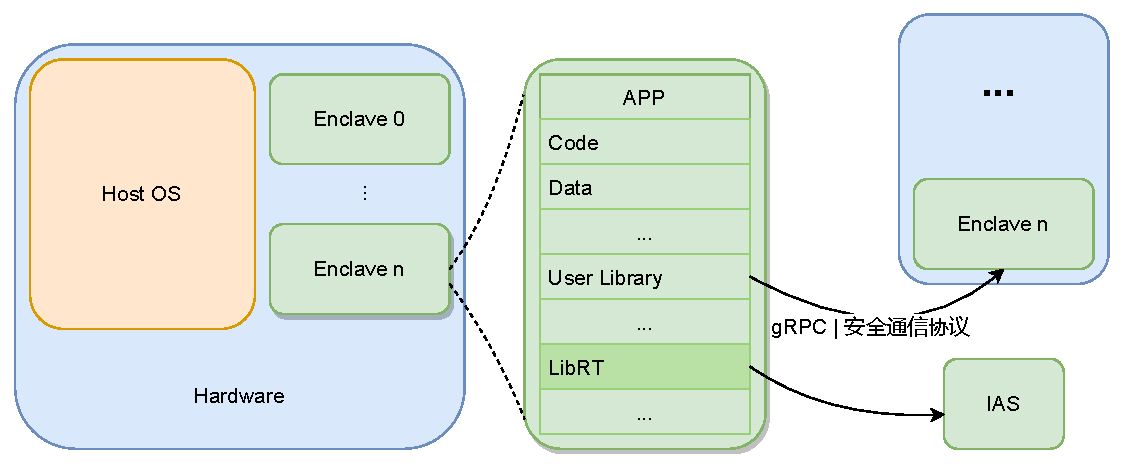
\includegraphics[width=.8\textwidth]{figures/architecture.pdf}
    \caption{平台总体架构图}
    \label{fig:architecture}
\end{figure}

图\ref{fig:architecture}展示了平台的总体架构。最外层的框代表硬件基础,其上运行着操作系统和安全飞地(Enclave)。将Enclave放大,内部运行着使用Rust语言编写的微服务节点程序,其结构类似于普通的进程,但是在库区域会有特殊的运行时库,提供操作系统相关功能的支持。
% ;但是我们同时借鉴了Rust-SGX的思想,在编译阶段将一些操作利用Rust-SGX提供的编译方法编译进程序中,这样可以减少对OS的依赖,从而可以进一步缩减Graphene为Rust-SGX不能支持的功能集合。我们将Rust-SGX不能支持的部分划分为模块,开发者可以根据自己开发节点的需要选择需要的模块进行编译,由此得到了一个模块化、小TCB的运行时。

节点之间的通信使用本次设计的安全通信协议进行保护,同时节点还要借助IAS提供的远程验证机制对其他节点的身份等进行验证。上层应用层通过gRPC进行远程过程调用。

\subsection{运行时设计}

由于SGX是一种硬件层面的支持,虽然Intel官方提供了一套开发工具SGX SDK~\cite{costan2016intel},但是不能直接运行现有的应用程序,必须按照其SDK规范重新编写。这样移植程序过于困难,因此我们需要一个运行时来屏蔽底层的细节,提供POSIX的接口给开发者使用。

目前的运行时设计主要有两种思路。第一种是在SGX中运行一个小型的操作系统,比如Microkernel(例如Keystone~\cite{lee2020keystone}的运行时)或LibOS(例如Graphene-SGX~\cite{tsai2017graphene}、Occlum~\cite{shen2020occlum}等),这样可以在无改动或极少改动的情况下将现有程序运行在SGX中;但是这种方式包含较多的代码,具有较大的TCB,可能存在较多漏洞和较大的攻击面。第二种思路是针对特定编程语言编写SGX内的运行时库(例如Rust-SGX~\cite{wang2019towards}、GoTEE~\cite{ghosn2019secured}等),这样编译生成的程序类似于使用SGX SDK开发的程序,可以在SGX中直接运行,由此可以达到很小的额外TCB;但是这种方式需要针对每种编程语言进行开发,且有些操作系统功能的实现非常困难。

我们的设计思路是将两种思路结合起来,同时兼顾两种思路的优点。考虑到微服务的特点,由于微服务的每个节点都很小,一般只需要操作系统提供的部分功能(例如网络通信),因此可以将LibOS进行拆分,将语言运行时库不能支持的功能按模块划分,达到按需引入的效果;同时虽然微服务架构是异构性的,但是每个节点往往都是由一种编程语言编写的,因此牺牲运行时的多语言支持是合理的。具体来说,我们从Graphene中拆分出Rust-SGX不能支持的功能,并尽量划分为独立的模块,开发者首先使用Rust-SGX提供的工具链编译出Object文件,然后与Graphene拆分得到的需要的模块进行链接,最终得到可以在SGX中运行的程序。由此可以减少不必要的系统功能,从而减小TCB,最终减小了攻击面,提高了系统安全性。

\subsection{安全通信协议设计}

使用安全通信协议是为了解决安全计算微服务场景下通信上的挑战,主要包含用户端和服务端的验证、微服务节点间互相验证对方的身份和合法性、微服务节点间通信的机密性和完整性保障、依赖节点间授权合法性的验证等。因此,我们进行了以下设计:

\paragraph{用户端身份验证和鉴权}
即用户在使用服务功能时,服务端要对用户身份信息进行认证,并鉴定用户所具有的权限,以决定是否允许用户使用服务功能。这一问题其实是SOA固有的问题,目前已经有比较成熟的解决方案,例如OAuth2~\cite{oauth2spec}等。由于此问题不是本次研究主要面对的问题,因此本次设计暂不考虑。

\paragraph{微服务节点间互相验证对方的身份和合法性}
这一点主要是确认对方未被恶意篡改、身份合法且运行在合法的SGX飞地中。一般我们认定运行在SGX中的程序不会被篡改,因此这一验证的目的是确保对方节点已被SGX保护,并在加载进入SGX之前未遭到篡改。在这种情况下,为了减少远程验证的开销,我们可以只在新节点第一次通信时进行验证,元数据变更(例如重新启动、更新升级等)的节点视作新节点。由于SGX提供了强大的远程验证机制~\cite{intel-sgx-ra},足够达到我们的需求,因此我们可以在此机制的基础上完善设计。

具体来说,每个节点都会维护一个信任白名单(T),记录所有合法的节点的地址(IP和端口号)到身份信息(ID)的映射,ID包括其MRENCLAVE、MRSIGNER、公钥等;每次发送请求时都需要将自己的ID发送给对方,对方会检查其ID是否在T中,如果不在,则会发起SGX远程验证,验证通过后将其加入T。为了保障安全,通信双方应进行双向认证。由于节点重启或更新后会生成新的ID,因此会自动重新进行远程验证并更新T上的表项。为防止出现地址变化导致表中记录弃用,占用过多内存,可以适当限制T的大小,并使用最近最少使用(LRU)算法清理弃用项。由于平台不存在恶意泄露ID的后门,进出SGX的数据也都会进行加密,因此攻击者无法窃取或伪造ID,这一验证机制是安全的。

\paragraph{微服务节点间通信的机密性和完整性保障}
这种情况其实是网络通信固有的问题,但是由于微服务场景下额外增加了应用内部节点间的网络通信,扩大了网络攻击的攻击面;如果节点间通信不采取安全措施,攻击者就可以发起各种网络攻击。这一问题其实可以采用成熟的网络安全通信协议作为解决方案,例如使用TLS~\cite{8446}。但是TLS等方案需要在通信之前进行握手,造成额外的通信开销,即使使用最新的TLS1.3也需要1-RTT进行握手~\cite{8446};再次通信时无论是状态恢复还是重新握手都会造成额外的网络延迟,而使用0-RTT的状态恢复则条件苛刻且有重放攻击的安全隐患。

在微服务场景中,与TLS的传统使用场景(如HTTPS)相比,我们观察到了以下3点现象:

\begin{itemize}
    \item 一个微服务节点只会和有依赖关系的固定的节点进行通信,这些节点的数量远远少于Web应用下HTTPS面对的客户端数量。
    \item 一个微服务节点的生命周期很长,一般只在重启或更新时才会改变地址;而HTTPS面对的客户端一般只有几分钟的生命周期。
    \item 在有SGX保护的情况下,可以认为对称共享密钥(SK)是不会泄露的。
\end{itemize}

因此,我们可以在微服务场景下只在第一次通信时进行握手,保留SK,之后的通信都可以直接使用。但是与0-RTT不同的是,在微服务场景下我们是可以使用计数器来防备重放攻击的,而不会受到0-RTT方式下Anti-Replay~\cite{8446}等方式的限制。

具体来说,我们扩充信任白名单T,添加记录通信过的节点的SK和计数器,每次请求时先检查T中是否有对方的记录,如果没有则需要先与对方进行1-RTT握手,双方都将计算出的对称密钥加入自己的T中,握手后进行加密通信;如果已有记录,则可以跳过握手直接进行通信。正式通信时要加入SK加密的ID,并使用计数器防止重放攻击。由于平台不存在恶意泄露对称密钥的后门,攻击者无法窃取SK,这一通信机制是安全的;且因为避免了重复握手,这个方案是高效的。

另外,由于TLS和SGX远程验证都需要使用DHKE建立加密通信,如果简单的将两者直接结合,会导致冗余的握手,从而影响性能。经过之前的分析,安全通信的握手和SGX远程验证都只需要在第一次通信时进行一次,因此我们可以让二者使用相同的SK,从而将两种协议结合起来,只需要一次握手即可完成密钥协商和远程验证两部分功能。

\paragraph{依赖节点间授权的合法性}
这里是为了保障微服务节点间能够进行细粒度的认证和授权,以防止攻击者窃取授权造成隐私扩散。在4种不同的基于Token的验证思路中,只有Token交换的方式可以实现细粒度和更高级别的安全保障,虽然会带来额外的计算开销,但是作为聚焦于安全的研究,我们选择使用这种更安全的方案;同时因为微服务的瓶颈是通信开销,额外JWT计算带来的开销是很小的,因此这一方案是可行的。另外,这一点应该是建立在上层应用层协议的基础上,因此实现时应在微服务示例程序中实现。

在以上设计下,两个微服务节点第一次通信的示意如图\ref{fig:communication}所示:

\begin{figure}[!ht]
    \centering
    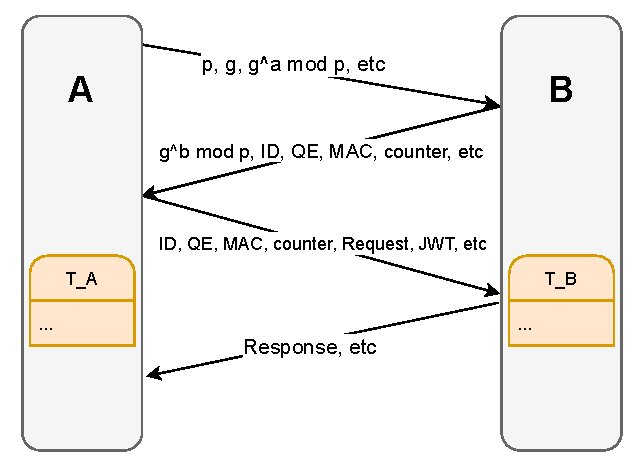
\includegraphics[width=.6\textwidth]{figures/communication.pdf}
    \caption{安全通信协议下第一次通信流程图}
    \label{fig:communication}
\end{figure}

\begin{enumerate}
    \item 请求方A检查自己的$T_A$中是否有被请求方B的记录,如果没有则进行DH握手(握手过程参考TLS1.3)。此时第一次通信一定没有记录,因此A发送握手请求,其中包含DH算法公开参数等信息。
    \item B收到A的DH公开参数,生成自己的DH算法参数,并返回握手响应。此时B已经可以计算得出SK,将其暂存;同时返回信息中包含SK加密的B的ID、QE和MAC,用于远程验证;返回信息中还有计数器等信息。
    \item A收到B的DH公开参数,计算出SK,并解密得到B的ID、QE、MAC和计数器。此时A要做2层检查:(1) 检查计数器值是否合法,如果合不合法则拒绝请求;(2) 检查自己的T中是否有B的记录,如果没有则向IAS发起验证,若IAS验证不通过则拒绝请求。2层检查之间没有先后关系,因此为了加快速度可以考虑并行验证。2层检查都通过后,A在$T_A$中生成以B的地址为键的记录,并填写SK、B的ID和计数器值等信息。接着A向B发送加密的请求信息,其中包含计数器值、A的ID、QE、MAC、用上级节点传入的JWT加工得到的新JWT(如有)、请求内容等数据。
    \item B收到请求后,也要进行2层验证。如果验证都通过,则在$T_B$中生成以A的地址为键的记录,填写SK、A的ID和计数器值等信息,并将请求内容发送给上层应用层协议(例如gRPC、HTTP)处理。应用层需要负责检查JWT中的身份和授权是否合法且有相应的权限,并根据授权情况执行处理(有可能继续和下级微服务进行通信);处理完成后,B将SK加密的结果返回给A。
    \item A接收到通信响应,解密得到通信结果,通信完成。
\end{enumerate}

总体来说,我们借鉴了TLS 1.3和SGX远程验证协议,将TLS的认证部分替换为由SGX的IAS进行远程验证,由此保证了通信的机密性、完整性和身份正确性;同时我们使用白名单的映射、SGX的内存保护和重新设计的验证流程,保证了双方身份信息和密钥的安全性,以及握手和验证的高效性。

\subsection{微服务示例程序设计}\label{subsec:ms-example}

为了后续实验验证我们的设计,我们还要设计一个简单的微服务示例程序。由于Rust~\cite{rust-lang}是一种新兴的编程语言,目前还没有使用Rust语言编写的开源微服务应用;已有的其他语言实现的微服务基准(例如DeathStarBench~\cite{gan2019open}和$\mu$Suite~\cite{sriraman2018mu}等)难以用Rust重写,且不是很符合安全计算的场景特点。因此,我们针对微服务安全计算的场景,设计了一个简单的图像处理相关的微服务示例程序,如图\ref{fig:ms-demo}所示。该示例程序共包含5个微服务节点,分别是:

\begin{figure}[!ht]
    \centering
    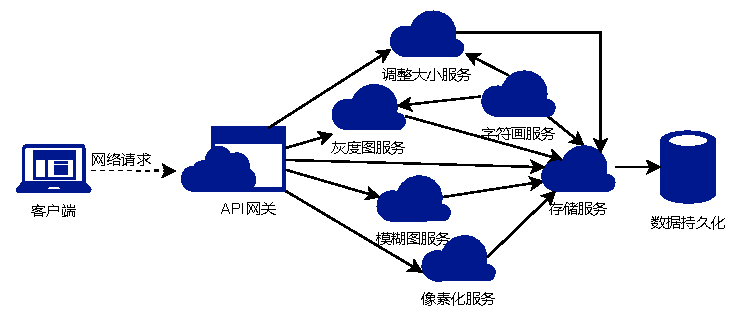
\includegraphics[width=.6\textwidth]{figures/msdemo.pdf}
    \caption{RPC流程图}
    \label{fig:ms-demo}
\end{figure}

\begin{itemize}
    \item \textbf{API网关节点}:用于和用户进行交互,接收用户的请求,将请求转发给下级的微服务节点,并将下级节点的响应返回给用户。
    \item \textbf{灰度图服务节点}:将传入图片处理为灰度图的节点。
    \item \textbf{字符画服务节点}:依赖于灰度图处理节点,将灰度图进一步处理为字符画的节点。
    \item \textbf{模糊图服务节点}:将传入图片进行模糊化处理的节点。
    \item \textbf{存储服务节点}:将数据库处理进行抽象,与数据持久化节点进行交互的节点。所有节点都可以将请求转发过来进行存储,但是由于不能保证数据库的安全性,在这里需要判断JWT中的授权信息,只有拥有存储权限的特殊用户才能够存取持久化的数据。
    \item \textbf{数据持久化节点}:运行数据库实例的节点,由于不是本项目开发的,不被信任假设包含,因此不能保证安全性。
\end{itemize}

该示例虽然简单,但是足够展示基本的微服务架构模型,并可以体现我们设计的多个方面(例如需要细粒度的授权管理)。为了微服务节点间通信的高效性,我们设计使用gRPC协议进行通信。
